% SC2008 --- Chapter 2: Application Layer (HTTP, DNS, Socket) --- 0->100 ground-up
\chapter{Application Layer: HTTP, DNS, and Sockets}
\label{ch:application}

\begin{quote}
\emph{``The Web is not the Internet.''} --- The Internet moves bytes; applications give them meaning. HTTP lets you fetch a page, DNS translates names to addresses, and sockets are the door between your program and the network. This chapter builds all three from intuition to working code.
\end{quote}

\noindent\fbox{\parbox{\dimexpr\linewidth-2\fboxsep-2\fboxrule}{%
\textbf{From zero: we build here, no sockets or Web background needed.} We define every application concept from scratch---processes, client--server, messages, names, sockets---with everyday analogies before formalism. Intuition comes first, then the definition, then the wire format and Python code. The only prerequisites are SC1004/SC2000 as in Ch.~1; no prior networking or systems programming is assumed.}}

\section*{Learning Outcomes}
After this chapter you will be able to:
\begin{enumerate}[label=(L\arabic*)]
    \item distinguish application architectures (client--server vs.\ peer-to-peer) and address a process via IP plus port;
    \item describe HTTP message formats, methods, status codes, and persistent versus non-persistent connections;
    \item explain DNS as a hierarchical, distributed database and trace iterative versus recursive resolution;
    \item use the socket API to build simple UDP and TCP client--server programs in Python;
    \item reason about cookies, Web caching, and conditional GET for performance.
\end{enumerate}

% ============================================================
\section{Principles: Processes, Sockets, and Transport Services}
\label{sec:app-principles}
An application is two \emph{processes} (running programs) talking over the network. The Web's two processes are \emph{browser} (client) and \emph{server}; BitTorrent's processes are peers. To find a remote process you need its host's \emph{IP address} and the process's \emph{port number} (like a building address plus an apartment number). A \emph{socket} is the programming interface between the application and the transport layer---think of it as the door through which the app pushes messages out and receives messages in.

What does an app need from transport? Four questions: (i) reliable delivery? (file transfer yes, live voice can tolerate loss); (ii) throughput guarantee? (video needs a minimum rate); (iii) timing guarantee? (games need low delay); (iv) security? (now almost always via TLS). The Internet offers two transport services: \emph{TCP} (reliable, ordered, congestion-controlled, connection-oriented) and \emph{UDP} (unreliable, no frills, faster). Applications choose: HTTP, mail, and file transfer use TCP; DNS and streaming often use UDP.

\begin{definition}[Client--server and P2P]
In \emph{client--server}, the server has a well-known address and is always on; clients contact it and do not talk to each other directly. In \emph{peer-to-peer}, peers are intermittently on and communicate directly with minimal server help, trading scalability for management complexity.
\end{definition}

This is the end-to-end argument again: the network core (IP) stays simple; reliability, if needed, is implemented at the edges by TCP inside the end hosts.

\begin{remark}[Choosing the right API]
If you need every byte delivered (Web, mail, remote login), pick TCP and pay its handshake and congestion-control overhead. If you need speed and can handle loss yourself (DNS, VoIP, gaming), pick UDP and add only the reliability you need. HTTP/3 intentionally runs over QUIC (reliable) on top of UDP to combine both worlds.
\end{remark}

% ============================================================
\section{The Web and HTTP}
\label{sec:http}
Intuition first: HTTP is like ordering at a restaurant. You (client) send a \emph{request} (``GET /menu'') and the kitchen (server) returns a \emph{response} (``200 OK'' plus the menu). The menu is an \emph{object} (HTML file, image, video) addressed by a \emph{URL}. Each object needs one fetch.

Two flavours of connection: \emph{non-persistent} opens a fresh TCP connection per object and closes it---simple but pays TCP handshake per object. \emph{Persistent} (default since HTTP/1.1) reuses one TCP connection for many objects, and \emph{pipelining} can send the next request before the prior response arrives.

\begin{figure}[h]
\centering
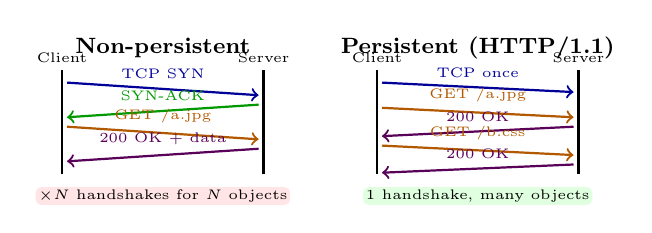
\begin{tikzpicture}[scale=0.80, every node/.style={font=\scriptsize}]
% Non-persistent timeline
\begin{scope}
\node[font=\footnotesize\bfseries] at (1.6,2.0) {Non-persistent};
\draw[thick] (0,0) -- (0,1.65); \draw[thick] (3.2,0) -- (3.2,1.65);
\node[font=\tiny] at (0,1.85) {Client}; \node[font=\tiny] at (3.2,1.85) {Server};
\draw[->, thick, blue!60!black] (0.08,1.45) -- (3.12,1.25) node[midway, above, font=\tiny] {TCP SYN};
\draw[->, thick, green!60!black] (3.12,1.10) -- (0.08,0.90) node[midway, above, font=\tiny] {SYN-ACK};
\draw[->, thick, orange!70!black] (0.08,0.75) -- (3.12,0.55) node[midway, above, font=\tiny] {GET /a.jpg};
\draw[->, thick, violet!70!black] (3.12,0.40) -- (0.08,0.20) node[midway, above, font=\tiny] {200 OK + data};
\node[font=\tiny, fill=red!10, rounded corners=2pt, inner sep=1pt] at (1.6,-0.35) {$\times N$ handshakes for $N$ objects};
\end{scope}
% Persistent timeline
\begin{scope}[xshift=5.0cm]
\node[font=\footnotesize\bfseries] at (1.6,2.0) {Persistent (HTTP/1.1)};
\draw[thick] (0,0) -- (0,1.65); \draw[thick] (3.2,0) -- (3.2,1.65);
\node[font=\tiny] at (0,1.85) {Client}; \node[font=\tiny] at (3.2,1.85) {Server};
\draw[->, thick, blue!60!black] (0.08,1.45) -- (3.12,1.30) node[midway, above, font=\tiny] {TCP once};
\draw[->, thick, orange!70!black] (0.08,1.05) -- (3.12,0.90) node[midway, above, font=\tiny] {GET /a.jpg};
\draw[->, thick, violet!70!black] (3.12,0.75) -- (0.08,0.60) node[midway, above, font=\tiny] {200 OK};
\draw[->, thick, orange!70!black] (0.08,0.45) -- (3.12,0.30) node[midway, above, font=\tiny] {GET /b.css};
\draw[->, thick, violet!70!black] (3.12,0.15) -- (0.08,0.02) node[midway, above, font=\tiny] {200 OK};
\node[font=\tiny, fill=green!12, rounded corners=2pt, inner sep=1pt] at (1.6,-0.35) {1 handshake, many objects};
\end{scope}
\end{tikzpicture}
\caption{HTTP with non-persistent versus persistent TCP. Persistence amortises the handshake; pipelining overlaps requests. Time flows downward.}
\label{fig:http-persistent}
\end{figure}

HTTP messages are plain text. A request has: request line (\texttt{GET /index.html HTTP/1.1}), headers (\texttt{Host:}, \texttt{Connection:}), blank line, optional body. A response has: status line (\texttt{HTTP/1.1 200 OK}), headers, body. Status families: \texttt{2xx} success, \texttt{3xx} redirect, \texttt{4xx} client error, \texttt{5xx} server error. Methods: \texttt{GET} fetches, \texttt{POST} submits, \texttt{PUT} stores, \texttt{DELETE} removes; \texttt{GET} is idempotent and cacheable.

\begin{lstlisting}[language=Python, caption={Minimal HTTP exchange with sockets---what the browser does.}]
import socket
s = socket.socket(socket.AF_INET, socket.SOCK_STREAM)
s.connect(("example.com", 80))  # TCP handshake happens here
req = "GET / HTTP/1.1\r\nHost: example.com\r\nConnection: close\r\n\r\n"
s.sendall(req.encode())
resp = b""
while chunk := s.recv(4096):
    resp += chunk
print(resp[:600].decode(errors="ignore"))
s.close()
# Persistent would reuse s for multiple GETs before close.
\end{lstlisting}

\emph{Cookies} let a stateless HTTP remember you: server sends \texttt{Set-Cookie}, browser stores it and replays on future requests. Cookies carry shopping carts, logins, and tracking---useful but privacy-sensitive. \emph{Web caching} (proxy) keeps a copy closer to you; a conditional GET with \texttt{If-Modified-Since} returns \texttt{304 Not Modified} if cached copy is fresh, saving bandwidth.

\begin{example}[Conditional GET saves bytes]
Your browser caches \texttt{logo.png} with \texttt{Last-Modified: Wed, 21 Aug 2026 07:00:00 GMT}. Next request sends \texttt{If-Modified-Since: Wed, 21 Aug 2026 07:00:00 GMT}. If the file is unchanged the server replies \texttt{304} with no body---a few hundred bytes instead of 50~KB. If modified, it replies \texttt{200 OK} with the new bytes.
\end{example}

% ============================================================
\subsection{HTTP Performance Tricks}
Beyond persistence, HTTP uses \emph{pipelining} (send next request before prior response arrives) and, in HTTP/2, \emph{multiplexing} many streams over one connection. A \emph{Content Delivery Network} replicates popular objects at edge caches nearer to you. Together they hide latency: the first fetch pays RTTs, later fetches hit the cache at LAN speed.

\section{DNS: The Internet's Phone Book}
\label{sec:dns}
You type \texttt{www.ntu.edu.sg}; the network needs an IP like \texttt{155.69.0.1}. \emph{DNS} is the distributed, hierarchical database that translates names to addresses (and more). Why not one central table? A single server would be a single point of failure, a traffic bottleneck, and far from many clients.

Hierarchy first: the name \texttt{www.ntu.edu.sg} reads right to left---root ($\cdot$), top-level domain (\texttt{sg}), second-level (\texttt{edu}), host (\texttt{www}). Each level is served by its own \emph{authoritative} name servers. A \emph{recursive resolver} (usually run by your ISP or 8.8.8.8) does the legwork; your host asks the resolver, which iteratively queries root $\to$ TLD $\to$ authoritative, caching answers along the way.

\begin{figure}[h]
\centering
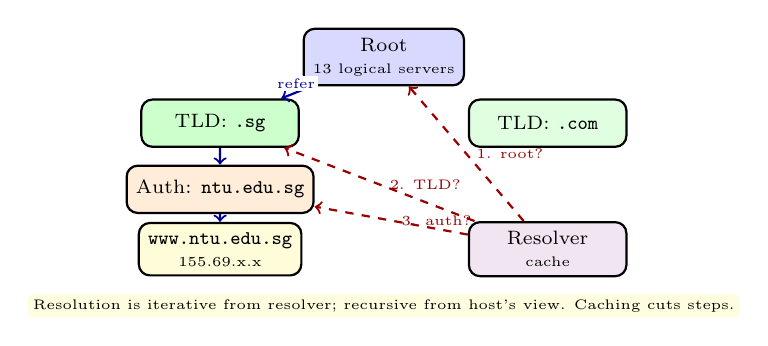
\begin{tikzpicture}[scale=0.80, every node/.style={font=\scriptsize},
  dns/.style={draw, thick, rounded corners=4pt, minimum width=2.0cm, minimum height=0.60cm, align=center}]
\node[dns, fill=blue!15] (root) at (0,2.4) {Root \\ \tiny 13 logical servers};
\node[dns, fill=green!20] (tld) at (-2.6,1.35) {TLD: \texttt{.sg}};
\node[dns, fill=green!12] (tld2) at (2.6,1.35) {TLD: \texttt{.com}};
\node[dns, fill=orange!15] (auth) at (-2.6,0.30) {Auth: \texttt{ntu.edu.sg}};
\node[dns, fill=yellow!15] (host) at (-2.6,-0.65) {\texttt{www.ntu.edu.sg}\\ \tiny 155.69.x.x};
\node[dns, fill=violet!10] (resolver) at (2.6,-0.65) {Resolver\\ \tiny cache};
\draw[->, thick, blue!60!black] (root) -- (tld) node[midway, above, font=\tiny, fill=white, inner sep=1pt] {refer};
\draw[->, thick, blue!60!black] (tld) -- (auth);
\draw[->, thick, blue!60!black] (auth) -- (host);
\draw[->, thick, red!60!black, dashed] (resolver) -- (root) node[midway, right, font=\tiny] {1. root?};
\draw[->, thick, red!60!black, dashed] (resolver) -- (tld) node[midway, right, font=\tiny] {2. TLD?};
\draw[->, thick, red!60!black, dashed] (resolver) -- (auth) node[midway, right, font=\tiny] {3. auth?};
\node[font=\tiny, align=center, fill=yellow!12, rounded corners=2pt, inner sep=2pt] at (0,-1.55) {Resolution is iterative from resolver; recursive from host's view. Caching cuts steps.};
\end{tikzpicture}
\caption{DNS hierarchy and resolution. The host asks its resolver once (recursive); the resolver walks the hierarchy iteratively. Each level delegates to the next via NS records.}
\label{fig:dns-hierarchy}
\end{figure}

DNS records are the rows: \texttt{A} (name $\to$ IPv4), \texttt{AAAA} (IPv6), \texttt{NS} (who is authoritative), \texttt{CNAME} (alias), \texttt{MX} (mail). Messages normally ride over \emph{UDP} (one query, one reply, fast); zone transfers use TCP. Caching and \texttt{TTL} (time to live) trade freshness for speed---exactly the consistency trade-off you will meet in databases (SC2207).

\begin{lstlisting}[language=Python, caption={DNS lookup in two lines---and a manual UDP query.}]
import socket
print(socket.gethostbyname("www.ntu.edu.sg"))  # uses OS resolver

# Manual: crafting a minimal DNS query is possible with dnspython or raw bytes
# but gethostbyname shows the abstraction: name in, address out.
# Underneath it sent a UDP datagram to port 53 and parsed the A record.
\end{lstlisting}

% ============================================================
\subsection{DNS Performance and Security}
DNS caching makes the Internet fast: once your resolver learns \texttt{ntu.edu.sg}, the next query for any host under it reuses the TLD and authoritative NS records. \emph{TTL} trades speed for freshness---short TTL means faster updates but more queries. Security matters: vanilla DNS has no authentication, so an attacker can spoof replies; \emph{DNSSEC} adds signatures so you can verify the answer really came from the authoritative server.

\section{Socket Programming: Doors to the Network}
\label{sec:sockets}
A socket is the API between application and transport. You create one, bind or connect, then send/receive. The crucial difference: \emph{UDP sockets} are connectionless---\texttt{sendto(address)} names the destination each time, like mailing a letter. \emph{TCP sockets} are connection-oriented---\texttt{connect(address)} first, then \texttt{send/recv} like a phone call, with a separate socket per accepted client on the server.

\begin{figure}[h]
\centering
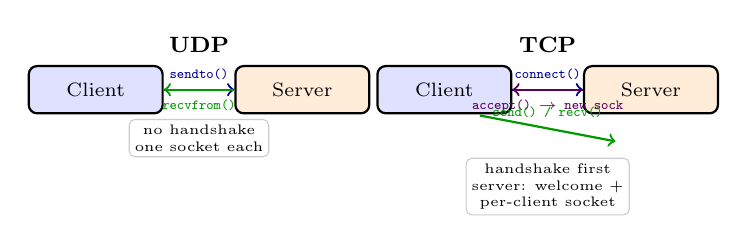
\begin{tikzpicture}[scale=0.82, every node/.style={font=\scriptsize}]
% UDP
\begin{scope}
\node[font=\footnotesize\bfseries] at (1.6,2.15) {UDP};
\node[draw, thick, fill=blue!12, rounded corners=3pt, minimum width=1.7cm, minimum height=0.60cm] (uc) at (0,1.45) {Client};
\node[draw, thick, fill=orange!15, rounded corners=3pt, minimum width=1.7cm, minimum height=0.60cm] (us) at (3.2,1.45) {Server};
\draw[->, thick, blue!60!black] (uc) -- (us) node[midway, above, font=\tiny] {\texttt{sendto()}};
\draw[->, thick, green!60!black] (us) -- (uc) node[midway, below, font=\tiny, dashed] {\texttt{recvfrom()}};
\node[font=\tiny, align=center, fill=white, draw=gray!40, rounded corners=2pt, inner sep=2pt] at (1.6,0.70) {no handshake\\one socket each};
\end{scope}
% TCP
\begin{scope}[xshift=5.4cm]
\node[font=\footnotesize\bfseries] at (1.6,2.15) {TCP};
\node[draw, thick, fill=blue!12, rounded corners=3pt, minimum width=1.7cm, minimum height=0.60cm] (tc) at (0,1.45) {Client};
\node[draw, thick, fill=orange!15, rounded corners=3pt, minimum width=1.7cm, minimum height=0.60cm] (ts) at (3.2,1.45) {Server};
\draw[->, thick, blue!60!black] (tc) -- (ts) node[midway, above, font=\tiny] {\texttt{connect()}};
\draw[->, thick, violet!70!black] (ts) -- (tc) node[midway, below, font=\tiny] {\texttt{accept() $\to$ new sock}};
\draw[->, thick, green!60!black] (0.55,1.05) -- (2.65,0.65) node[midway, above, font=\tiny] {\texttt{send() / recv()}};
\node[font=\tiny, align=center, fill=white, draw=gray!40, rounded corners=2pt, inner sep=2pt] at (1.6,-0.05) {handshake first\\server: welcome +\\per-client socket};
\end{scope}
\end{tikzpicture}
\caption{UDP versus TCP sockets. UDP is message-oriented and connectionless; TCP is byte-stream, connection-oriented, one new socket per client.}
\label{fig:socket-udp-tcp}
\end{figure}

\begin{lstlisting}[language=Python, caption={UDP echo and TCP echo---the two minimal client--servers.}]
# --- UDP server (connectionless) ---
import socket
us = socket.socket(socket.AF_INET, socket.SOCK_DGRAM)
us.bind(("", 12000))
while True:
    data, addr = us.recvfrom(2048)
    us.sendto(data.upper(), addr)   # echo uppercased

# --- UDP client ---
# cs = socket.socket(socket.AF_INET, socket.SOCK_DGRAM)
# cs.sendto(b"hello", ("127.0.0.1", 12000))
# print(cs.recvfrom(2048)[0])

# --- TCP server (connection-oriented, one socket per client) ---
# vs = socket.socket(socket.AF_INET, socket.SOCK_STREAM)
# vs.bind(("", 12001)); vs.listen(1)
# while True:
#     conn, addr = vs.accept()      # new socket conn
#     data = conn.recv(1024)
#     conn.sendall(data.upper())
#     conn.close()
\end{lstlisting}

Pitfalls: TCP is a \emph{byte stream}---one \texttt{send} may need multiple \texttt{recv}s; always loop. UDP datagrams are bounded ($\approx$1472~bytes before IP fragmentation). Close sockets or you leak ports. Use \texttt{SO\_REUSEADDR} during development so restarts do not hit ``Address already in use.''

% ============================================================
\begin{remark}[Stateless but not memoryless]
HTTP itself remembers nothing between requests (stateless), yet cookies and server-side sessions add memory above it. This split keeps the protocol simple while letting applications be stateful---another instance of the end-to-end principle. Caches must be careful: a cached copy of a bank balance must not be served to another user; \texttt{Cache-Control: private} prevents that.
\end{remark}

\section{Chapter Notes}
HTTP evolution: 1.0 (non-persistent), 1.1 (persistent, caching, cookies), 2 (multiplexed streams), 3 (QUIC over UDP). Fielding's REST dissertation formalised HTTP semantics. DNS is RFC~1034/1035; DNSSEC adds authentication. Sockets are Berkeley (1983); Beej's Guide remains the practical companion. Try Wireshark to watch HTTP and DNS live.

% ============================================================
\section{Exercises}
\label{sec:ch02-exercises}
\begin{enumerate}[label=E2.\arabic*, leftmargin=*, itemsep=0.8em]
    \item \textbf{HTTP timing.} A page has base HTML (4000~bytes) plus 4 images (each 8000~bytes). Non-persistent HTTP needs one TCP handshake (1~RTT) plus one request/response per object. Persistent reuses one handshake. If RTT$=20$~ms and link rate is large, compare total time for both. How does pipelining help?
    \item \textbf{Status and methods.} A browser fetches \texttt{/a.html} and gets \texttt{301 Moved: Location /b.html}, then fetches \texttt{/b.html} and gets \texttt{200 OK} plus \texttt{Set-Cookie: id=7}. Explain each step, whether \texttt{GET} or \texttt{POST} is appropriate to submit a login form, and where the cookie is stored and replayed.
    \item \textbf{DNS walk.} Starting with an empty resolver cache, trace queries to resolve \texttt{mail.ntu.edu.sg}: which servers are contacted in order, what record types are returned, and where caching helps the next query for \texttt{www.ntu.edu.sg}? Contrast iterative versus recursive from the host's viewpoint.
    \item \textbf{Socket bytes vs.\ messages.} A TCP client does \texttt{send(b"HELLO")} once; the server loops \texttt{recv(2)} five times. What might each \texttt{recv} return, and why is this impossible with UDP? Write the correct TCP receive loop that reassembles exactly 5~bytes.
    \item \textbf{Caching and consistency.} A Web cache stores \texttt{/data.json} with \texttt{TTL}=60~s. A client requests it at $t=0, 30, 80$~s while the origin updates at $t=50$~s. Which requests hit the cache and what do they return? How does \texttt{If-Modified-Since} with \texttt{304} reduce cost when TTL expires but the object has not changed?
\end{enumerate}
% End of Chapter 2